\chapter{Design Evaluation}\label{chap:eval}

This section outlines the tests used to validate the greenhouse systems setup and operation. It includes performance tests to validate selection and design of sensors, actuators the system as a whole and its wireless monitoring and control capabilities. 

\section{Sensor Validation}\label{sec:sensor_validation}

All sensors were tested to verify their response and accuracy to real environmental changes under controlled conditions.  Each was connected to the ESP32 microcontroller with the appropriate pin configuration, and real-time data was logged at one-second intervals through serial communication. 
The data was imported into MATLAB for processing and visualization. 
This setup ensured consistent testing and provided clear insight into each sensor’s performance characteristics.

\subsection{Temperature and Humidity Sensor (DHT22)}

\subsubsection*{Test Objective}
The purpose of this test was to verify the accuracy and responsiveness of the DHT22 sensor to real environmental changes in temperature and humidity. 

\subsubsection*{Methodology}
The sensor was connected to the ESP32 microcontroller through serial comunication and live readings were recorded. 
A burst of warm air was directed towards the sensor to simulate a rapid change in environmental conditions. 
The corresponding temperature and relative humidity values were logged and plotted using MATLAB for analysis. 

\subsubsection*{Results}
The plotted data, shown in Figure~\ref{fig:dht22_test}, demonstrates the sensor's response to the applied stimulus. 
A clear rise in temperature was observed immediately after exposure to warm air, accompanied by a corresponding change in humidity. 

\begin{figure}[H]
	\centering
	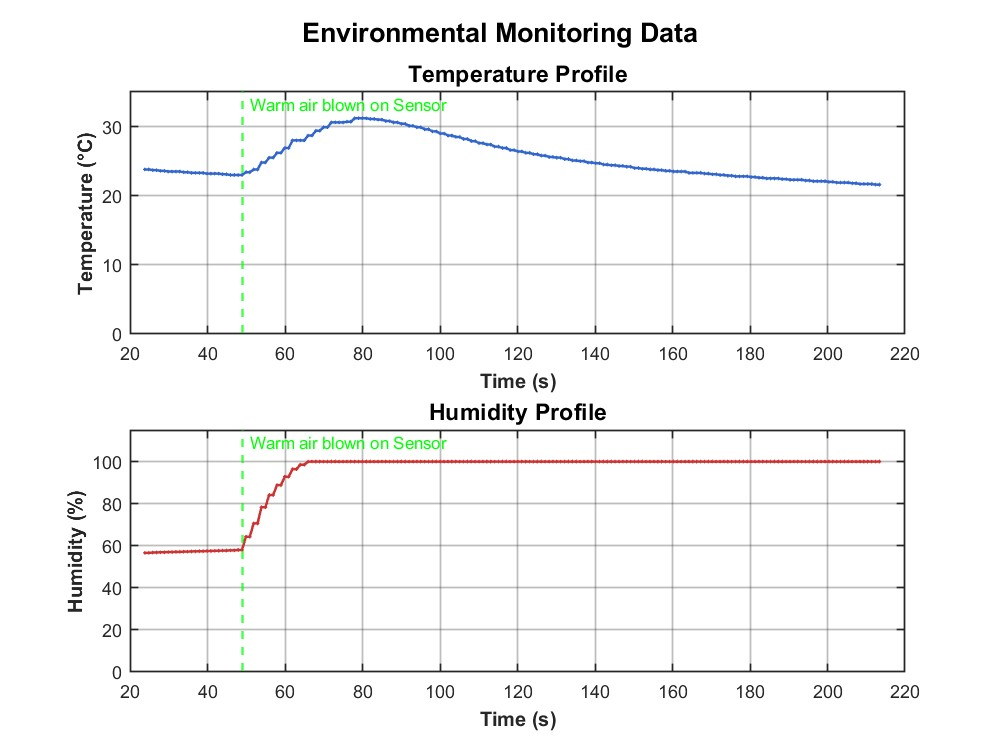
\includegraphics[width=0.7\textwidth]{figs/dthtest.jpg}
	\caption{DHT22 response to applied warm air (temperature and humidity vs. time).}
	\label{fig:dht22_test}
\end{figure}

\subsubsection*{Discussion}
The test confirms that the DHT22 sensor responds promptly to changes in environmental conditions, with smooth and continuous data output. 
The test showed the expected rise in both temperature and humidity. 
However, it was noted that the humidity readings temporarily saturated at the maximum percentage due to condensation forming within the sensor. 
After a short period, the values gradually returned to ambient levels. 
While this behavior is not ideal, it is a known characteristic of the sensor under extreme conditions and is not expected to cause issues during normal greenhouse operation, where such rapid condensation is unlikely to occur. 
Slight response delays were also noted, which are consistent with the DHT22's documented sampling rate and latency.

\subsection{Summary of Additional Sensor Tests}

Following the same testing approach described above, all sensors were validated for responsiveness and reliability. 
Each test involved controlled exposure to changing environmental conditions, with data recorded via serial communication and analyzed in MATLAB. 
A summary of key results is provided below, as the procedures followed were identical to those of the DHT22 test.

\subsubsection*{Soil Moisture Sensor}
The sensor was connected to the ESP32 microcontroller through ADC and real‑time values were logged. The sensor probes were sequentially tested in open air, damp soil, and fully submerged conditions. 
As shown in Figure~\ref{fig:soilmoisture_test}, the readings ranged from approximately \(0\%\) in dry air to \(80\%\) when submerged, demonstrating clear distinction between soil moisture states. 
The sensor provided consistent and repeatable readings, confirming its suitability for automated irrigation control. The calibration process will ensure more accurate mapping of percentage values to volumetric water content, but the results demonstrate strong baseline performance for the intended application.

\begin{figure}[H]
	\centering
	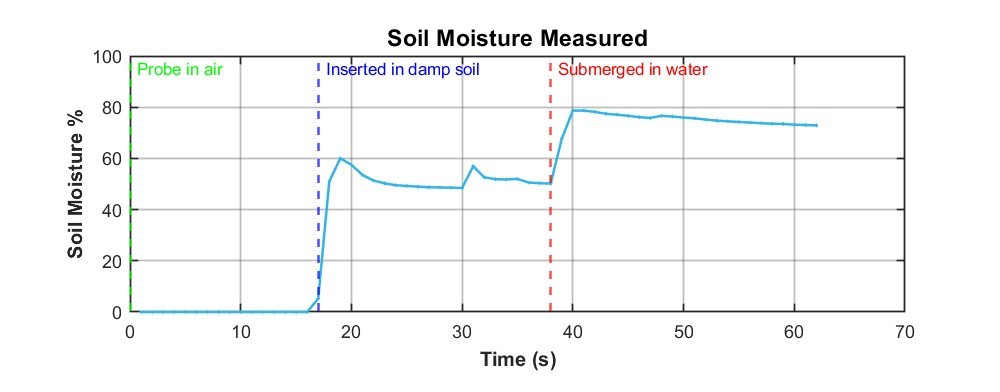
\includegraphics[width=0.8\textwidth]{figs/soiltest.jpg}
	\caption{Soil moisture sensor response in open air, damp soil, and submerged in water.}
	\label{fig:soilmoisture_test}
\end{figure}

\subsubsection*{Light Sensor}
The BH1750 light sensor was connected to the ESP32 via the I2C interface, and its lux readings were logged in real time. The sensor was exposed to varying illumination using a handheld torch. 
As seen in Figure~\ref{fig:bh1750_test}, the sensor responded sharply, rising from 40\,lux (ambient) to approximately 200\,lux under direct illumination, then returning to baseline upon removal of the light source. 
This confirmed its accuracy and responsiveness to dynamic lighting conditions. 

\begin{figure}[H]
	\centering
	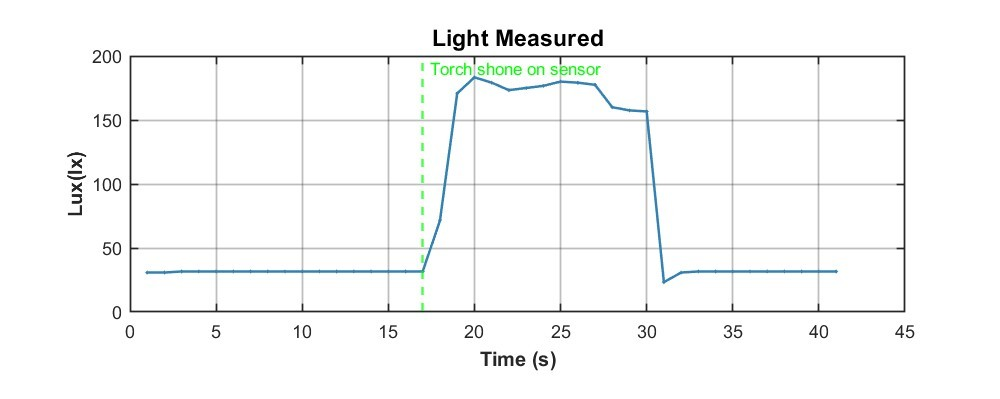
\includegraphics[width=0.7\textwidth]{figs/lighttest2.jpg}
	\caption{BH1750 light sensor response to torch illumination and return to ambient lighting.}
	\label{fig:bh1750_test}
\end{figure}

\subsubsection*{CO\textsubscript{2} Sensor}
The MHZ19B CO\textsubscript{2} sensor was connected to the ESP32 via UART communication and its readings were logged in real time. The sensors readings were allowed to stabilize at ambient indoor conditions (approximately 1000\,ppm) before being exposed to a burst of exhaled air. 
The concentration rapidly increased to the sensor’s limit of 5000\,ppm, then decayed back to baseline within two minutes, as shown in Figure~\ref{fig:co2_response}. 
This validated the sensor’s sensitivity, recovery time, and overall suitability for environmental monitoring.

\begin{figure}[H]
	\centering
	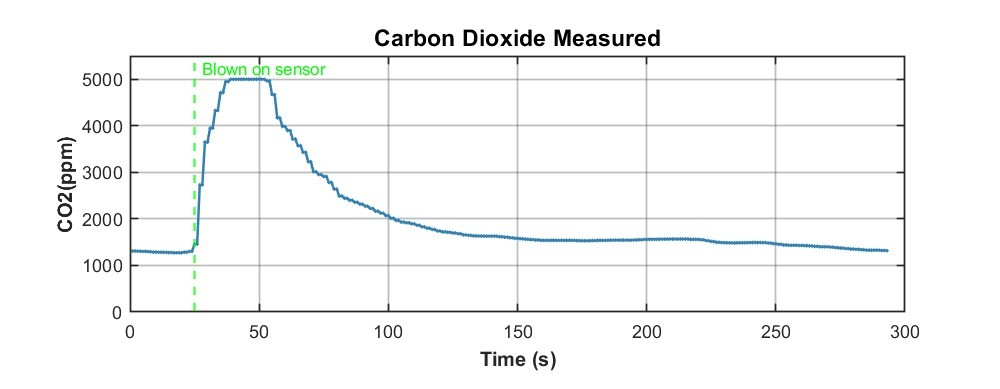
\includegraphics[width=0.7\textwidth]{figs/CO2test.jpg}
	\caption{CO\textsubscript{2} sensor response to rapid change in concentration.}
	\label{fig:co2_response}
\end{figure}

\subsection*{Summary Discussion}
Across all tests, the sensors exhibited expected and reliable responses to environmental variations. 
Minor latency and saturation effects observed under extreme conditions are consistent with manufacturer specifications and are not expected to affect normal operation. 
The results confirm that all selected sensors are well-suited for integration into the automated greenhouse control system.

\section{Actuator Validation }

Each actuator was connected to its respective relay channel, corresponding to the assigned GPIO pin on the microcontroller. 
Testing was carried out by first supplying the rated voltage directly to each actuator, followed by validation through relay control. 
A logical HIGH signal was written to each GPIO pin to trigger the relay, with successful activation confirmed visually via the built-in indicator LED and audibly by the distinct clicking sound of the relay switch. 
As the relay module operates in active-high mode, actuators were connected to either the Normally Open (NO) or Normally Closed (NC) terminals as required. 
Once verified, the appropriate 5\,V or 12\,V supply was connected to the Common (CO) port to power the actuators. 
Table~\ref{tab:actuator_tests} summarizes the testing procedures and outcomes for each actuator.

\begin{table}[H]
	\centering
	\caption{Actuator Testing and Observations}
	\label{tab:actuator_tests}
	\begin{tabular}{|p{3cm}|p{6cm}|p{6cm}|}
		\hline
		\textbf{Actuator} & \textbf{Test Procedure} & \textbf{Observation} \\
		\hline
		Solenoid Valve & 12\,V applied directly, then via relay control. Bulk and high-frequency capacitors added to suppress voltage spikes. & Audible switching confirmed; misting nozzles activated and deactivated with relay control. \\
		\hline
		Linear Actuator & 12\,V applied with polarity switching, then via relay-controlled H-bridge. & Extension and retraction observed correctly in both directions. Relay control verified reliable actuation. \\
		\hline
		Supplemental Lighting & 12\,V applied directly, then switched via relay control. & Purple UV grow light switched on and off reliably under both direct and relay control. \\
		\hline
		Intake / HAF Fans & 12\,V applied directly, then via relay control. & Fans powered on successfully; airflow observed. Relay switching confirmed proper operation. \\
		\hline
	\end{tabular}
\end{table}

With the mains water supply connected, the solenoid valve successfully controlled the misting system, providing adequate pressure to the misting nozzles. The nozzles were observed to start and stop spraying water in direct response to the relay switching.

During testing, it was observed that switching the misting solenoid simultaneously with Wi-Fi activity (e.g., ThingSpeak uploads) introduced supply transients that caused the ESP32 to briefly brown-out and reset. The solenoid’s inductive kickback and relay contact bounce injected noise onto the 12 V rail, which coupled into the 5 V supply. To mitigate this, a bulk electrolytic capacitor and a high-frequency ceramic capacitor were added at the solenoid driver terminals. These components damped the transient response and provided local energy buffering, resulting in stable system operation without timeouts or resets.

\section{Remote monitoring}

\subsection{Objective}
The objective of this experiment was to verify the successful implementation of remote monitoring and user control for the greenhouse system. The aim was to confirm that environmental parameters could be measured, transmitted, stored, and visualized in real time through wireless platforms, and that user-defined setpoints could be remotely updated.

\subsection{Methodology}
The test was conducted using the ESP32 microcontroller configured to interface with two IoT platforms: \textit{ThingSpeak} and \textit{Blynk}.  
For remote monitoring, the ESP32 was programmed to upload data for all environmental parameters including temperature, humidity, soil moisture, CO\textsubscript{2}, and light intensity at 20-second intervals to the ThingSpeak cloud platform. A custom dashboard was developed to visualize these readings in real time, as shown in Figure~\ref{fig:Wireless Monitoring Dashboard}.  

For remote control, the system was integrated with the Blynk IoT platform. A mobile dashboard was created (Figure~\ref{fig:Blynk}) to enable the user to adjust key control parameters such as temperature and humidity setpoints through sliders and buttons. . The ESP32 was connected to Eduroam services and configured with a unique
Blynk template and authentication token, allowing remote updates of setpoints for various environmental parameters.

\subsection{Results}
The greenhouse successfully transmitted all sensor data to ThingSpeak without communication interruptions. The online dashboard updated at the programmed 20-second interval, confirming the reliability of wireless data transfer and cloud visualization. Historical data was logged and plotted on the ThingSpeak channel, verifying successful storage for later analysis, as presented in Section~\ref{sec:response}.

\begin{figure}[H]
	\centering
	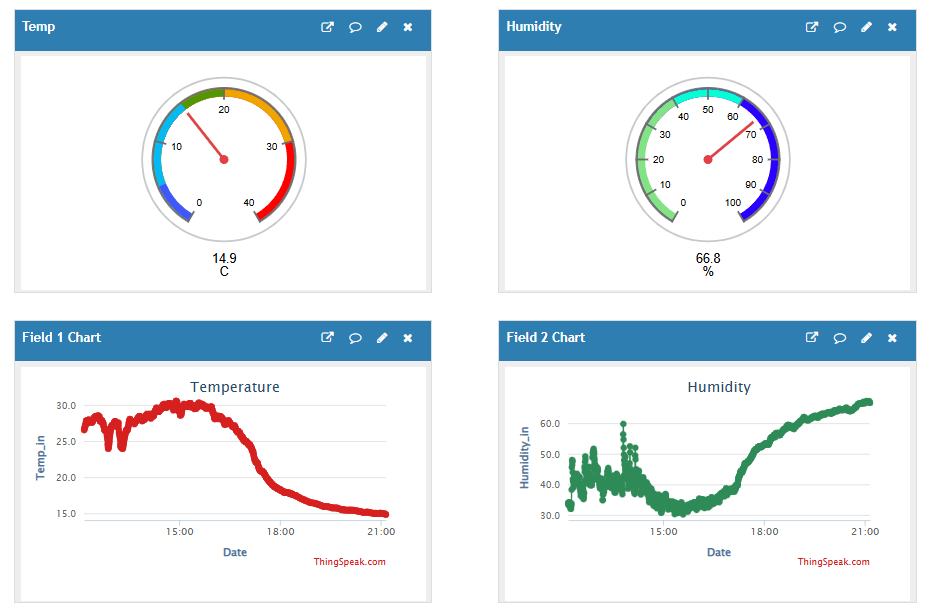
\includegraphics[width=0.7\textwidth]{figs/dash.png}
	\caption{Wireless Monitoring Dashboard.}
	\label{fig:Wireless Monitoring Dashboard}
\end{figure}


The Blynk dashboard enabled real-time modification of environmental setpoints from a mobile device. Commands sent via Blynk were received by the microcontroller with negligible delay. Parameter changes were reflected in the system's behaviour, demonstrating successful two-way communication between the user and the greenhouse.

\begin{figure}[H]
	\centering
	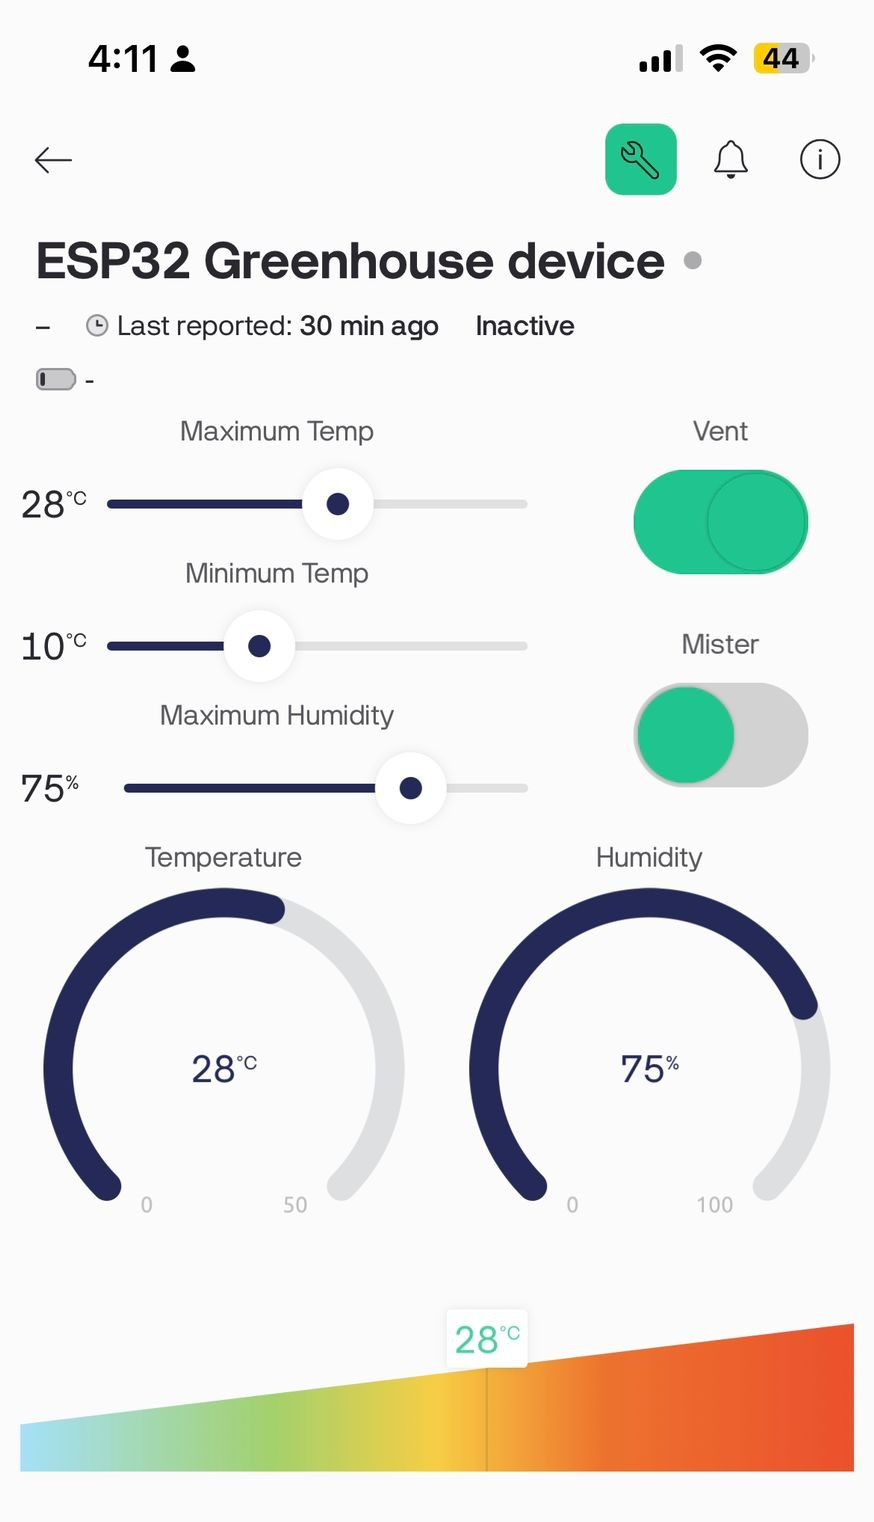
\includegraphics[width=0.35\textwidth]{figs/blynk.jpeg}
	\caption{User App with Blynk}
	\label{fig:Blynk}
\end{figure}


\subsection{Discussion}
The experiment confirmed that both remote data monitoring and user interaction were successfully achieved. While ThingSpeak proved effective for real-time data visualization and long-term data storage, Blynk offered a more intuitive interface for real-time control adjustments. The combined use of these platforms allows both analytical monitoring and interactive management of greenhouse conditions.


\section{Solar Power Test}

To validate the capability of the solar subsystem to power the greenhouse entirely off-grid, a series of tests were conducted. The procedure was as follows:

\begin{enumerate}
	\item The battery voltage was measured with no load connected, showing 12.8\,V, indicating a partial state of charge (full charge is approximately 14.8\,V).  
	\item The battery was connected to the Skyking charge controller via the positive and negative terminals. Upon connection, the controller powered on and displayed the battery voltage.  
	\item Using the controller menu, the float voltage was set to 13.7\,V, the discharge stop voltage to 10.8\,V, and the battery type configured as a sealed gel battery, in accordance with the battery manufacturer’s recommended operating conditions.  
	\item The solar panels were connected using MC4 connectors. The charge controller confirmed successful charging through its display.  
	\item The 12\,V supply terminal block and greenhouse system ground were connected to the load terminals of the charge controller.  
	\item The controller display indicated power transfer to the load. This was verified by measuring the potential difference across the load terminals with a multimeter.  
\end{enumerate}

These steps confirmed correct wiring and successful operation of the solar power subsystem. The charge controller additionally provides low-voltage protection by disconnecting the load if the battery voltage drops below a safe threshold. During full system testing, it was confirmed that the solar array supplied sufficient power to operate the greenhouse without discharging the battery to unsafe levels even during days with high cloud cover.


\section{Greenhouse Setup}

The Full Greenhouse setup can be seen in the figure below. Please see Appendix \ref{chap:pics} for additional pictures.

\begin{figure}[H]
	\centering
	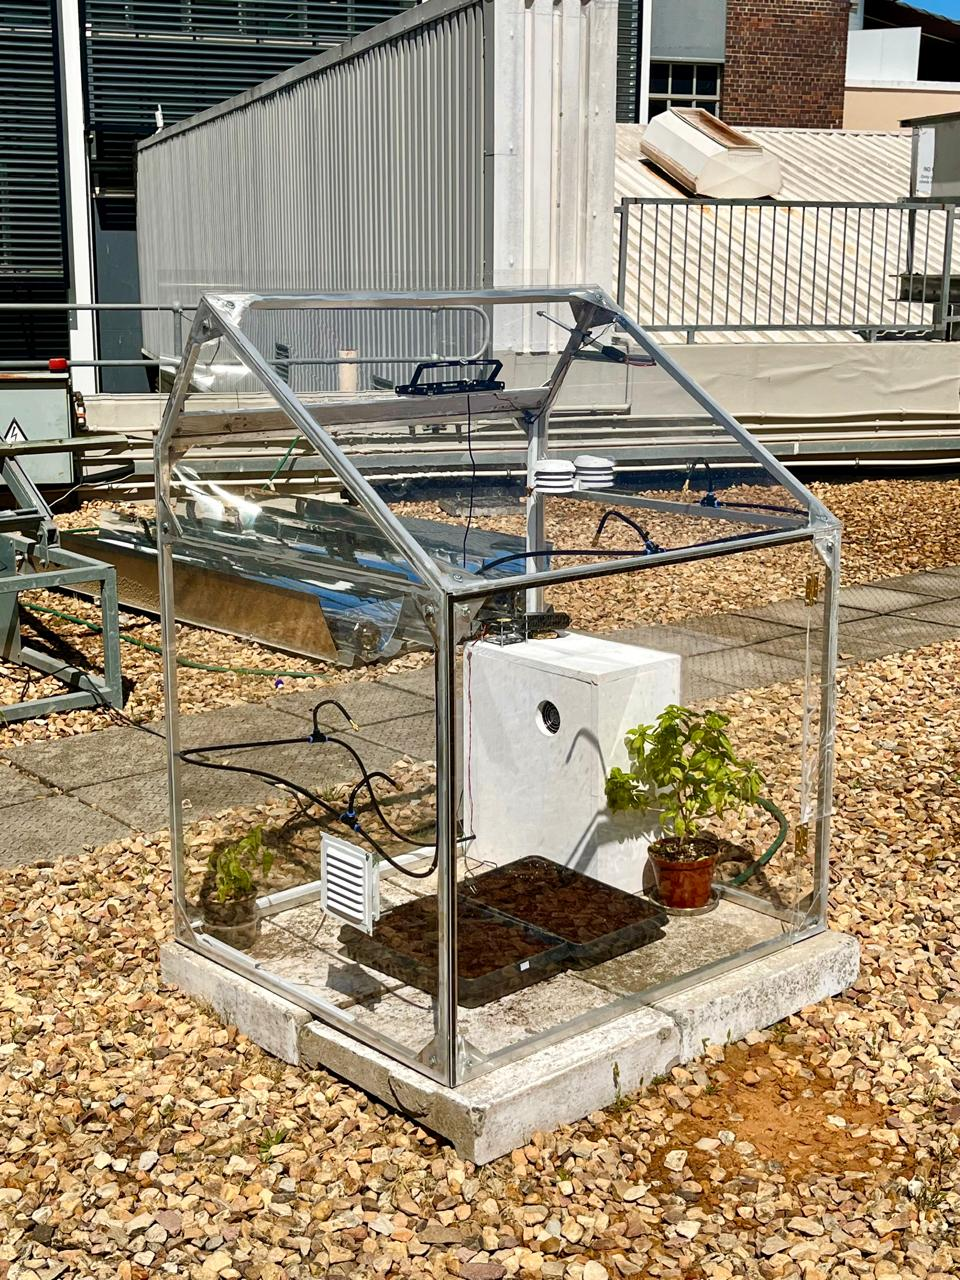
\includegraphics[width=0.4\textwidth]{figs/setup.jpeg}
	\caption{Greenhouse Setup}
	\label{fig:Greenhouse Setup}
\end{figure}

\section{Enviromental Response}\label{sec:response}

With all sensors, actuators, solar power components, and monitoring systems successfully tested, installed, and integrated, the complete greenhouse system can now be operated with all functions active. The system is powered on and allowed to continuously measure environmental conditions while autonomously regulating the internal climate toward the desired setpoints.

\subsection{ Dual Phase Test}

To evaluate the performance of the greenhouse control system, a two-phase test procedure was conducted. In the first phase, the greenhouse was operated for three full day–night cycles with all sensors and monitoring systems active, but without the actuators connected. This allowed the internal environment to respond passively to external conditions, providing a baseline measurement of natural fluctuations in temperature, humidity, and light.

In the second phase, the actuators (ventilation, irrigation, and heating) were connected and enabled. The greenhouse was again run for more than three full day–night cycles, with the control system actively attempting to regulate conditions towards the desirable setpoints. This phase demonstrates the effectiveness of the system in stabilizing the greenhouse environment.

The temperature, humidity and soil data from both phases were collected from Thingspeak and plotted using python, enabling a direct comparison between passive response and active control. The resulting figures highlight the extent to which the actuators improve environmental stability and overall system performance.

\begin{figure}[H]
	\centering
	\begin{subfigure}[b]{0.7\textwidth}
		\centering
		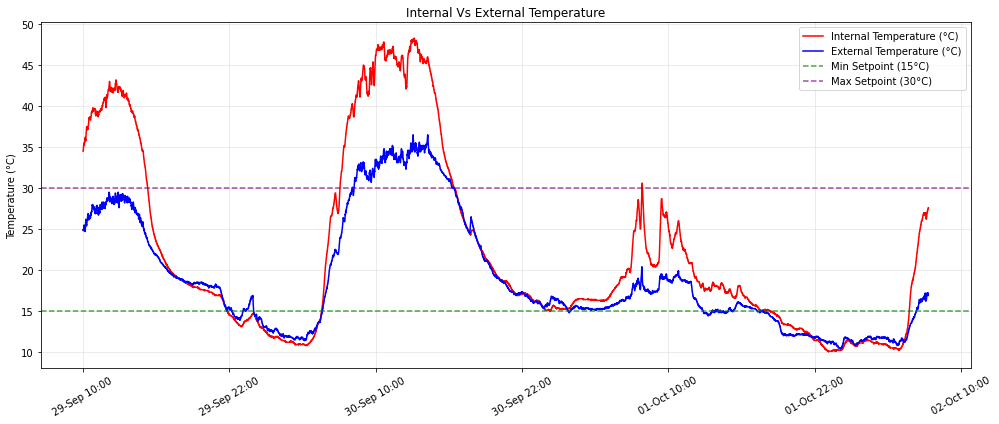
\includegraphics[width=\textwidth]{figs/temp_n.png}
		\caption{Actuators off}
		\label{fig:temp_off}
	\end{subfigure}
	\vskip\baselineskip
	\begin{subfigure}[b]{0.7\textwidth}
		\centering
		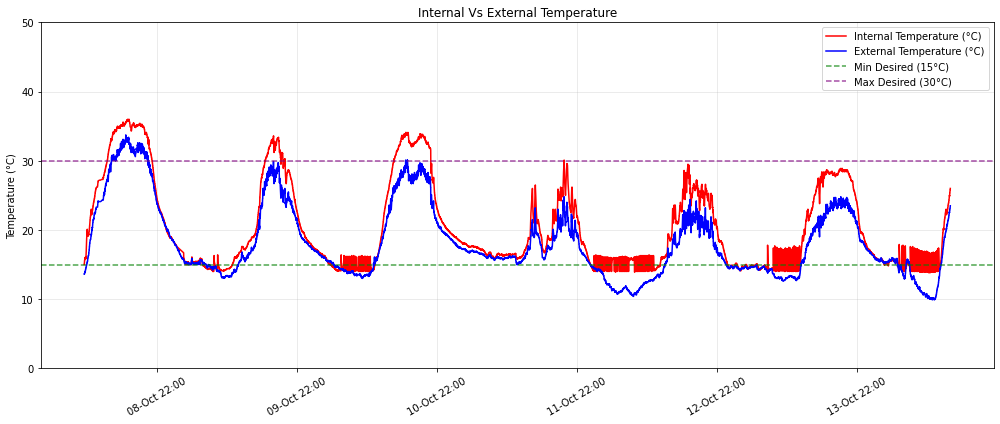
\includegraphics[width=\textwidth]{figs/temp_a.png}
		\caption{Actuators on}
		\label{fig:temp_on}
	\end{subfigure}
	\caption{Internal vs. external temperature profiles for the greenhouse with (a) Actuators off and (b) Actuators on.}
	\label{fig:temp_comparison}
\end{figure}


During the actuator-off test, the internal environment of the greenhouse was allowed to fluctuate naturally with ambient conditions. Without any active control, the internal temperature (shown in red) rose to a peak of approximately \SI{48}{\celsius} during the day, significantly exceeding optimal growing conditions. At night, the temperature dropped well below the desired setpoint, reaching approximately \SI{10}{\celsius}, highlighting the system’s vulnerability to external temperature extremes under passive operation.

In contrast, during the actuator-on test, the greenhouse exhibited an improved thermal response. The heating system successfully maintained the internal temperature near the desired setpoint of \SI{15}{\celsius} during cooler periods, keeping the environment consistently warmer than outside conditions. However, under hot daytime conditions, the system faced challenges in reducing internal temperatures, which remained around \SI{5}{\celsius} above ambient. Despite this limitation, the active ventilation, circulation fans, and misting system provided measurable cooling benefits compared to the uncontrolled scenario, in which temperatures rose to approximately \SI{15}{\celsius} above ambient due to the unchecked greenhouse effect heating the internal environment.

\begin{figure}[H]
	\centering
	\begin{subfigure}[b]{0.7\textwidth}
		\centering
		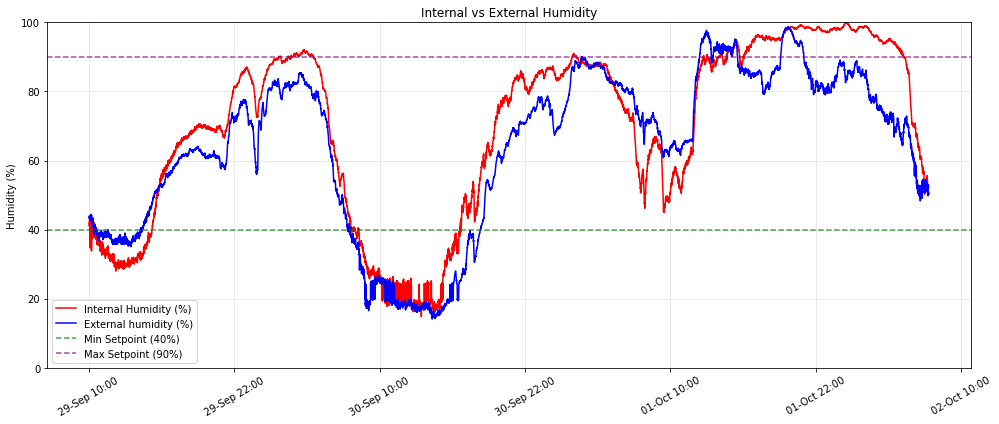
\includegraphics[width=\textwidth]{figs/hum_n.png}
		\caption{Actuators off}
		\label{fig:hum_off}
	\end{subfigure}
	\vskip\baselineskip
	\begin{subfigure}[b]{0.7\textwidth}
		\centering
		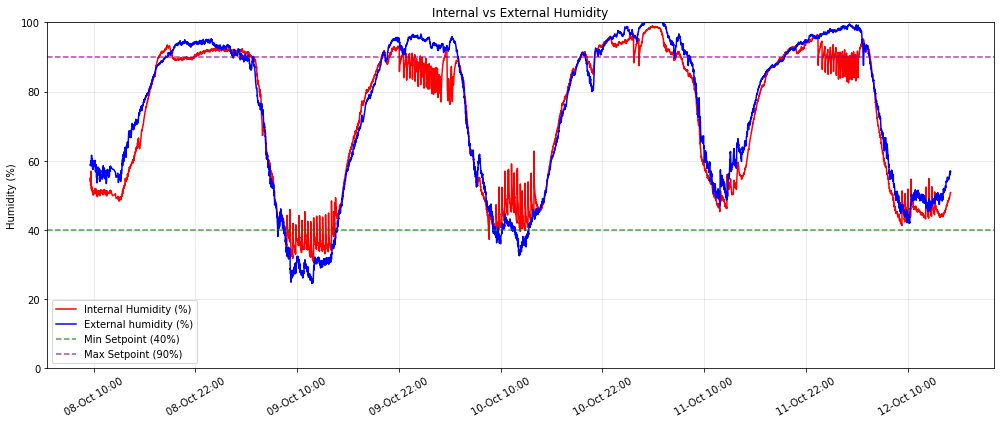
\includegraphics[width=\textwidth]{figs/hum_a.png}
		\caption{Actuators on}
		\label{fig:hum_on}
	\end{subfigure}
	\caption{Internal vs.\ external humidity profiles for the greenhouse with (a) actuators off and (b) actuators on.}
	\label{fig:hum_comparison}
\end{figure}


During the actuator-off phase, the internal and external humidity profiles closely mirrored one another, with relative humidity varying widely between 20\% and 100\% over the day–night cycle. This variation reflects the natural dependence of relative humidity on temperature, decreasing during the warmer daytime periods and increasing overnight.

When the actuators were enabled, the system responded to low humidity by activating the misting function every 20 minutes, visible as periodic spikes in the recorded data. These misting periods effectively restored the internal humidity to within the desired range, demonstrating successful environmental regulation. At night, operation of the heater caused a further decrease in humidity, an unintended but beneficial effect that prevented excessive condensation and maintained more balanced conditions during peak humidity levels. However, during times when the heater was inactive due to adequate internal temperatures, the humidity occasionally exceeded the desired maximum setpoint. 

Overall, the actuator-on phase exhibited a more stable humidity range of 40\% to 100\%, compared to the uncontrolled 20\% to 100\% range. While the system was unable to maintain the desired maximum humidity limit of 90\%, it successfully prevented humidity from dropping below 40\%, demonstrating effective intermittent misting control.

\begin{figure}[H]
	\centering
	\begin{subfigure}[b]{0.7\textwidth}
		\centering
		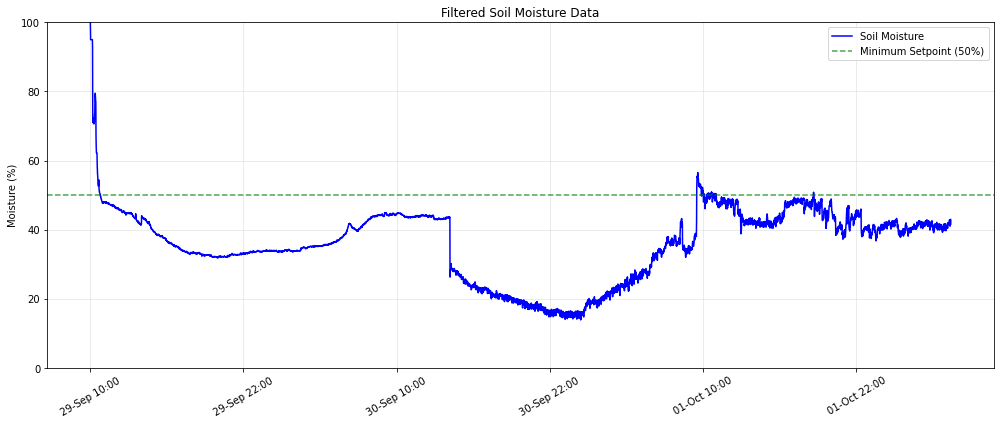
\includegraphics[width=\textwidth]{figs/soil_n.png}
		\caption{Actuators off}
		\label{fig:Soil_off}
	\end{subfigure}
	\vskip\baselineskip
	\begin{subfigure}[b]{0.7\textwidth}
		\centering
		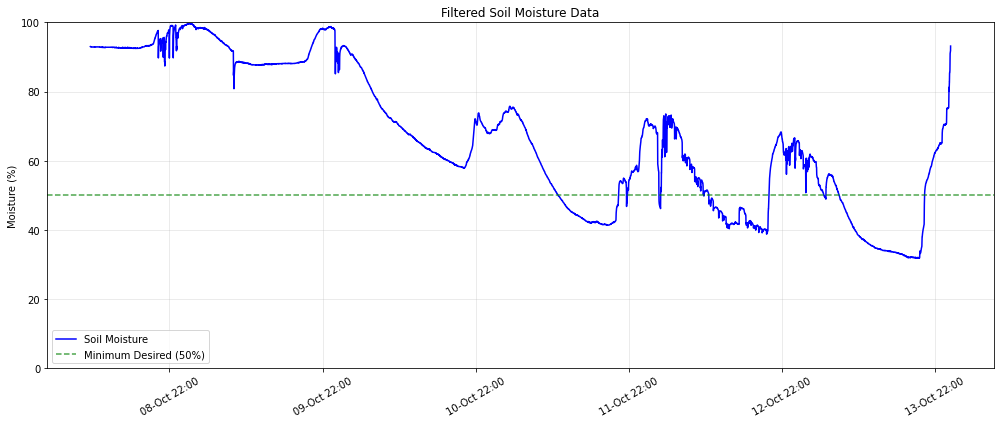
\includegraphics[width=\textwidth]{figs/soil_a.png}
		\caption{Actuators on}
		\label{fig:Soil_on}
	\end{subfigure}
	\caption{Soil Moisture profile for the greenhouse with (a) actuators off and (b) actuators on.}
	\label{fig:soil_comparison}
\end{figure}

During the initial phase, when the mister was inactive, the soil moisture content gradually declined and remained below the setpoint as the soil medium dried out. A slight increase was observed on the third day following a cold, rainy night, likely due to condensation re-entering the soil system.

When the actuators were enabled, the soil moisture stabilized around 70\% for several days before dropping below the setpoint, at which point the misting system activated to restore the desired moisture level. The data showed a recurring pattern of moisture loss during the night, followed by misting events during the day that raised levels above the setpoint. On average, the system maintained soil moisture within or slightly above the desired range, demonstrating effective control based on sensor feedback.

The fluctuations and response delays observed, are attributed to the misting system’s operational settings, restricted to daytime activation and governed by a duty cycle of two minutes on every twenty minutes, as described in Appendix~\ref{flow}. These constraints were intentionally implemented to prevent overwatering, allow time for sensor feedback stabilization, and avoid unintended nighttime cooling when thermal regulation takes priority.

\subsection{ CO\textsubscript{2} and Lux Observation}

\begin{figure}[H]
	\centering
	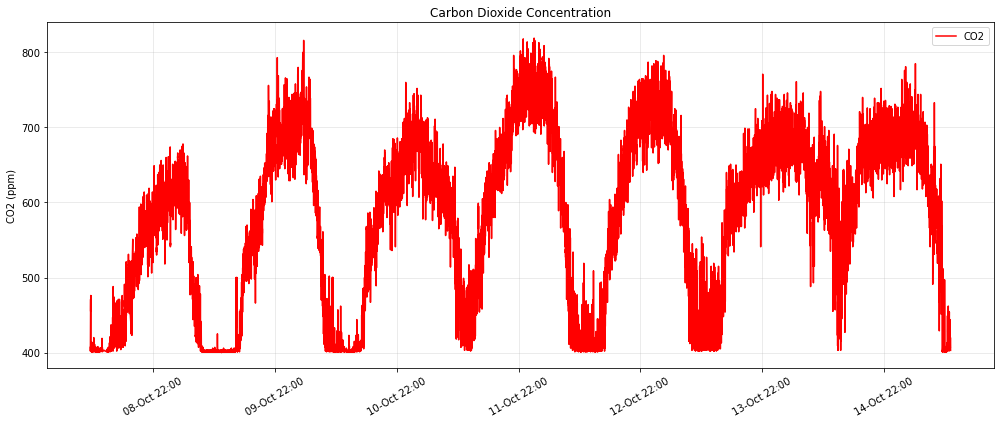
\includegraphics[width=0.7\textwidth]{figs/co2data.png}
	\caption{CO\textsubscript{2} Profile}
	\label{fig:CO2}
\end{figure}


The \(\mathrm{CO_{2}}\) plot provides valuable insight by highlighting a distinct day–night cycle, with concentrations rising during the night as a result of plant respiration. 
This trend is consistent with general ambient \(\mathrm{CO_{2}}\) behavior and does not indicate any problematic accumulation within the greenhouse. Since the levels remained within healthy ranges for plant growth, no active control or actuation was required, such as venting to regulate concentrations.  


\begin{figure}[H]
	\centering
	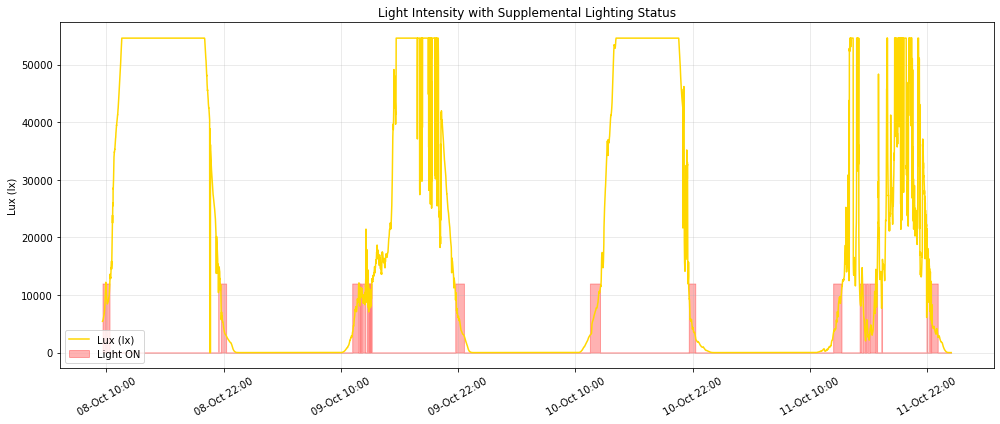
\includegraphics[width=0.7\textwidth]{figs/lux.png}
	\caption{Lux Profile}
	\label{fig:Lux}
\end{figure}

The plot of the light intensity profile illustrates the digital on/off state of the supplemental LED lighting. 
As calculated in Appendix~D, the LED was designed to provide 
\SI{200}{\micro\mole\per\square\meter\per\second} PPFD and was configured to activate whenever the ambient 
levels dropped below this threshold, but only during daylight hours. This corresponds to an illuminance of approximately 
\SI{10800}{lux}. The lighting can be observed switching on during the early morning and evening periods, as well as 
intermittently on the second day when cloud cover reduced incoming solar radiation.

\section{Evaluation Using Performance Requirements}

\begin{threeparttable}
	\caption{Performance Requirement Verification}\label{tab:performance_verification}
	\begin{tabular}{|p{1.5cm}|p{4.5cm}|c|p{3cm}|p{3cm}|}
		\hline
		\textbf{PR Number} & \textbf{Description} & \textbf{Target} & \textbf{Actual} & \textbf{Comment} \\
		\hline
		2 & Resist Wind speeds & 18.81\,kph & Not Tested & Validated through calculations \\
		\hline
		3 & Temperature sensing range & -10–50\,°C & -40–80\,°C & Passed \\
		\hline
		4 & Soil moisture sensing & 0–100\,\% & 0–100\,\%  & Passed \\
		\hline
		5 & Humidity sensing & 0–100\,RH\% & 0–100\,RH\%  & Passed \\
		\hline
		6 & CO\textsubscript{2} sensing range & 0–1000\,ppm & 0–5000\,ppm & Passed \\
		\hline
		7 & Light sensing & 0–600\,\si{\micro\mole\per\metre\squared\per\second} & 0–925\,\si{\micro\mole\per\metre\squared\per\second} & Passed \\
		\hline
		8 & Latency in displaying environmental conditions & <120\,s & $\sim$30\,s average & Passed \\
		\hline
		9 & Control temperature & 15 min–30 max\,°C & 15–35\,°C maintained & 15 min Passed - 30 max Failed \\
		\hline
		10 & Control soil moisture content & 50–100\,\% & 50–100\,\% maintained during day & Passed \\
		\hline
		11 & Control humidity & 40 min–90 max\,\% & 40–95\,\% maintained & 40 min Passed - 90 max Failed \\
		\hline
		12 & Supplemental lighting intensity & 200\,\si{\micro\mole\per\metre\squared\per\second} & Not tested & Validated through calculations \\
		\hline
		13 & Energy consumption & 0–1200\,Wh & 980\,Wh over 24\,h & Validated in calculations \\
		\hline
		14 & Battery storage capacity & >24\,h & Not Tested & Remained sufficiently charged through solar over cloudy periods \\
		\hline
	\end{tabular}
\end{threeparttable}


\section{Full system Test with Plants Growth}

The operational success of the greenhouse system was validated through a controlled two-week growth trial of microgreens, conducted to verify the system’s ability to maintain suitable environmental conditions for plant growth. The experiment served as a performance test against the design requirements related to temperature, humidity, and irrigation control. Four microgreen varieties (peas, radish, beetroot, and arugula) were planted within the greenhouse. As shown in the before-and-after photographs below, all varieties exhibited healthy germination and growth, confirming that the system effectively supported sustained plant development and met its intended functional objectives.

\begin{figure}[H]
	\centering
	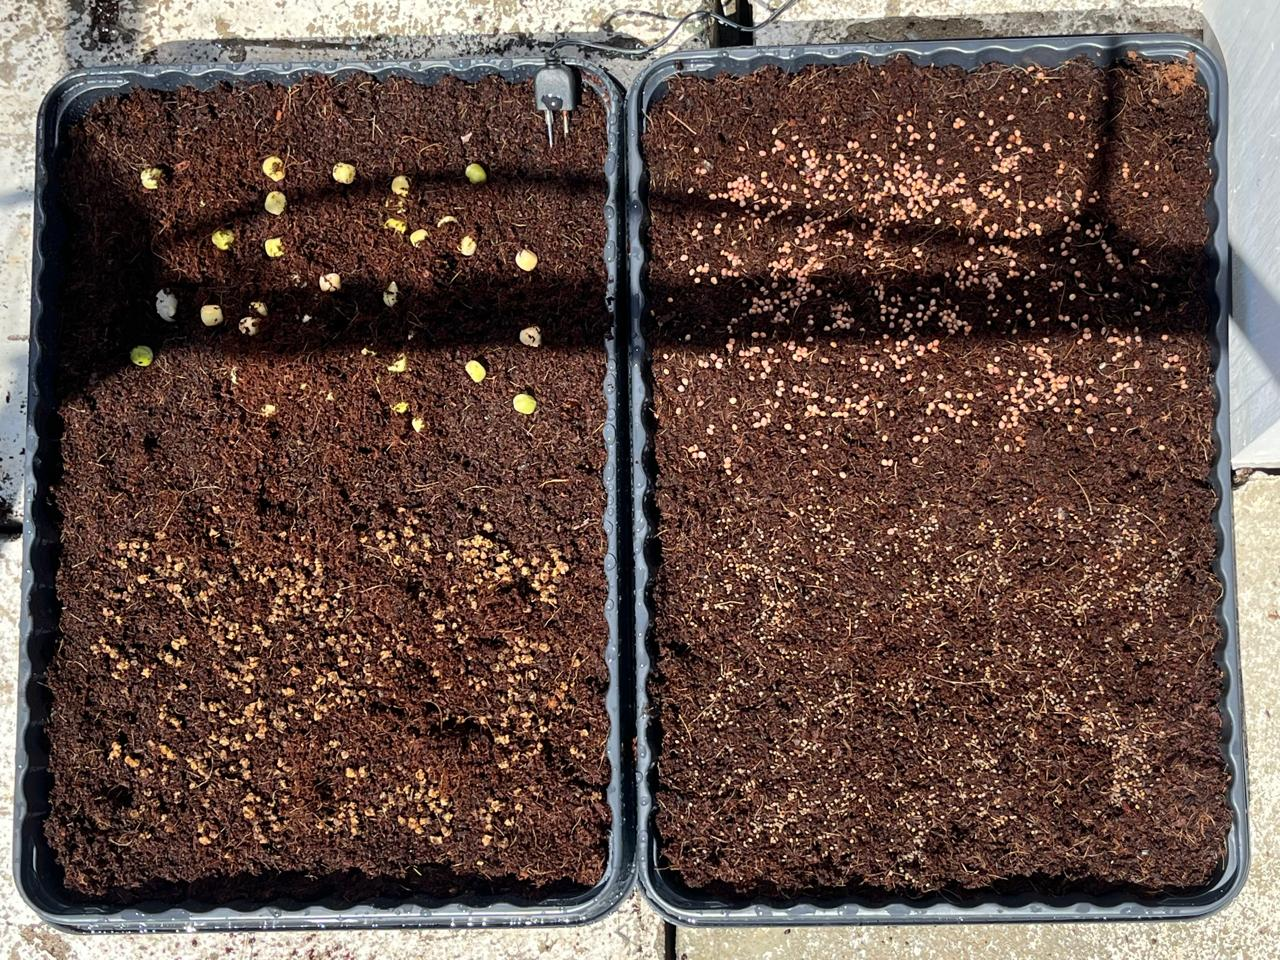
\includegraphics[width=0.7\textwidth]{figs/greens.jpeg}
	\caption{Microgreens Seeds}
	\label{fig:Microgreens}
\end{figure}

\begin{figure}[H]
	\centering
	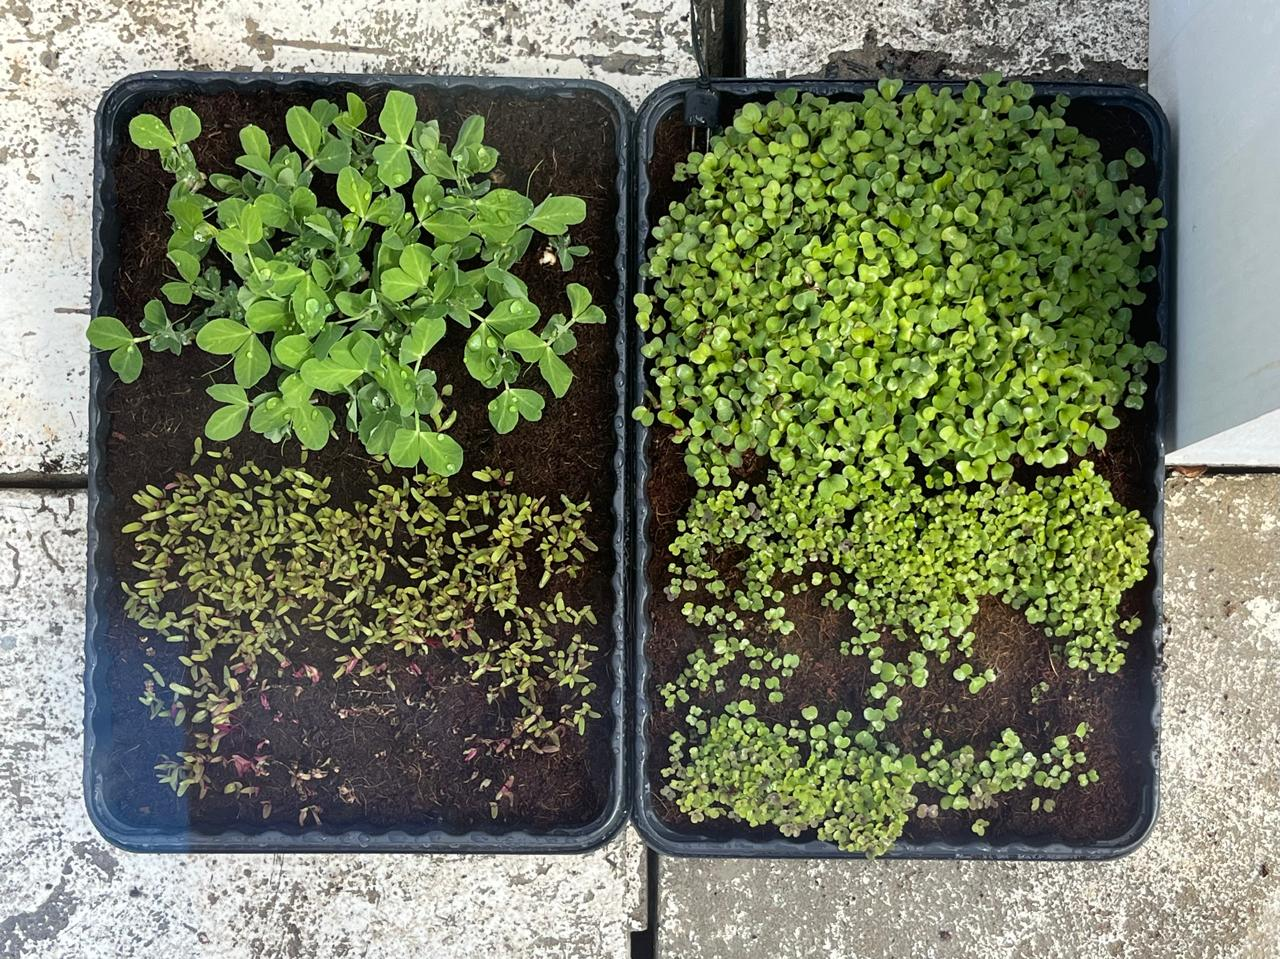
\includegraphics[width=0.7\textwidth]{figs/green2.jpeg}
	\caption{Microgreens}
	\label{fig:Microgreens}
\end{figure}

